% ============================================================
%  TruthfulRAG v5 — Viva Presentation  (5 slides + title)
%  Beamer + Madrid theme, custom IIIT-blue palette
%  Compile: pdflatex viva_presentation.tex  (twice)
% ============================================================
\documentclass[aspectratio=169, 10pt]{beamer}

\usetheme{Madrid}
\usecolortheme{whale}

\definecolor{iiitblue}{RGB}{0,51,102}
\definecolor{iiitgold}{RGB}{204,153,0}
\definecolor{lightgray}{RGB}{245,245,245}

\setbeamercolor{palette primary}   {bg=iiitblue,       fg=white}
\setbeamercolor{palette secondary} {bg=iiitblue!80,    fg=white}
\setbeamercolor{palette tertiary}  {bg=iiitblue!60,    fg=white}
\setbeamercolor{palette quaternary}{bg=iiitblue,       fg=white}
\setbeamercolor{structure}         {fg=iiitblue}
\setbeamercolor{alerted text}      {fg=iiitgold}
\setbeamercolor{block title}       {bg=iiitblue,       fg=white}
\setbeamercolor{block body}        {bg=lightgray,      fg=black}

\usepackage[T1]{fontenc}
\usepackage{lmodern}
\usepackage{booktabs}
\usepackage{array}
\usepackage{xcolor}
\usepackage{tikz}
\usepackage{amsmath}
\usepackage{colortbl}
\usepackage{multirow}

\newcolumntype{L}[1]{>{\raggedright\arraybackslash}p{#1}}
\newcolumntype{C}[1]{>{\centering\arraybackslash}p{#1}}
\newcommand{\rowV}{\rowcolor{iiitblue!15}}
\newcommand{\rowG}{\rowcolor{green!10}}
\newcommand{\rowR}{\rowcolor{red!10}}

\setbeamertemplate{navigation symbols}{}

% ── Metadata ─────────────────────────────────────────────
\title[TruthfulRAG v5]{\textbf{TruthfulRAG v5}\\[3pt]
  \small Conflict-Aware Knowledge-Graph RAG System}
\author[Eesh Saxena]{Eesh Saxena \quad 230101032 \quad B.Tech CSE \quad IIIT Manipur}
\date[April 2026]{Viva-Voce Presentation \quad April 2026}

% ============================================================
\begin{document}

% ── TITLE ───────────────────────────────────────────────────
\begin{frame}
  \titlepage
  \vspace{-6pt}
  \centering\scriptsize
  \textit{Based on arXiv:2511.10375 — implemented, extended, and evaluated}
\end{frame}

% ============================================================
% SLIDE 1 — Introduction, Objective & Contributions
% ============================================================
\begin{frame}{Slide 1 \quad Introduction, Objective \& Contributions}

\begin{columns}[T]
% ── Left: problem + objective ──────────────────────────────
\begin{column}{0.38\textwidth}
  \begin{block}{\small Problem \& Objective}
    \scriptsize
    \begin{itemize}\setlength\itemsep{2pt}
      \item LLMs \textbf{hallucinate} — confident wrong answers
      \item LangChain RAG cannot resolve \textbf{contradicting docs}
      \item 1985 doc = 2023 doc in retrieval score — \alert{no recency}
      \item No system gives a \textbf{confidence score}
    \end{itemize}
    \vspace{4pt}
    \textbf{Goal:} Implement KG-RAG v4, identify weaknesses,\\
    build v5 with 6 novel improvements, evaluate on 325 queries.
  \end{block}
\end{column}
% ── Right: contributions table ─────────────────────────────
\begin{column}{0.59\textwidth}
  \begin{block}{\small 6 Novel Contributions}
    \centering\scriptsize
    \begin{tabular}{cL{1.8cm}L{5.0cm}}
      \toprule
      \rowcolor{iiitblue}
      \textcolor{white}{\textbf{\#}} &
      \textcolor{white}{\textbf{Name}} &
      \textcolor{white}{\textbf{Formula / Mechanism}} \\
      \midrule
      \rowV N1 & Corroboration &
        Score $\times\;(1+\ln(1+\text{support})\times 0.8)$ \\[1pt]
      \rowV N2 & Temporal Decay &
        Score $\times\;e^{-0.08\times\text{age}}$
        — older facts score lower \\[1pt]
      \rowV N3 & Hybrid Retrieval &
        BM25 + Semantic, fused via RRF:
        $\tfrac{1}{60+r_\text{bm25}}+\tfrac{1}{60+r_\text{sem}}$ \\[1pt]
      \rowV N4 & Time Snapshots &
        Historical queries filter graph to that year only \\[1pt]
      \rowV N6 & Audit Trail &
        JSON log: which facts kept, removed, and why \\[1pt]
      \rowV N7 & Confidence &
        $0.40\,h + 0.30\,\text{sup} + 0.30\,\text{rec}$ (0–100\%) \\
      \bottomrule
    \end{tabular}
  \end{block}
\end{column}
\end{columns}

\end{frame}

% ============================================================
% SLIDE 2 — Background & Existing Work
% ============================================================
\begin{frame}{Slide 2 \quad Background \& Existing Work}

\begin{columns}[T]
% ── Left: comparison table ─────────────────────────────────
\begin{column}{0.55\textwidth}
  \centering\scriptsize
  \begin{tabular}{L{2.0cm}C{0.6cm}L{2.0cm}L{2.0cm}}
    \toprule
    \rowcolor{iiitblue}
    \textcolor{white}{\textbf{System}} &
    \textcolor{white}{\textbf{Yr}} &
    \textcolor{white}{\textbf{Approach}} &
    \textcolor{white}{\textbf{Limitation}} \\
    \midrule
    LangChain RAG  & 2020 & Chunk + cosine  & No conflict logic \\[1pt]
    Self-RAG       & 2023 & Self-critique   & No graph, no time \\[1pt]
    CRAG           & 2024 & Web fallback    & Intra-corpus blind \\[1pt]
    MADAM-RAG      & 2024 & Agent debate    & Majority vote only \\[1pt]
    \rowcolor{iiitgold!20}
    KG-RAG v4      & 2024 & Graph + entropy &
      \textbf{No year field; gap = 0.028} \\[1pt]
    \rowV \textbf{v5 (Ours)} & \textbf{26} &
      Decay + corroboration &
      \textbf{Gap = 1.126 → resolved} \\
    \bottomrule
  \end{tabular}
\end{column}
% ── Right: the key gap explained ───────────────────────────
\begin{column}{0.42\textwidth}
  \begin{block}{\small Why v4 Fails — The 0.028 Problem}
    \scriptsize
    \begin{tabular}{lcc}
      \toprule
      \textbf{Fact} & \textbf{v4} & \textbf{v5} \\
      \midrule
      \rowR SAFE\_FOR (1985)      & 1.133 & 0.592 \\
      \rowG CONTRAINDICATED (2023)& 1.161 & 1.718 \\
      \midrule
      Gap   & \alert{0.028} & \textbf{1.126} \\
      Result& \alert{Both reach LLM} & \textbf{Stale eliminated} \\
      \bottomrule
    \end{tabular}
    \vspace{4pt}

    Decay: $e^{-0.08\times16}=0.278$ (1985)\\
    vs $e^{-0.08\times3}=0.787$ (2023)\\[3pt]
    \alert{v4 threshold = 0.30} — gap too small\\
    \textbf{v5 gap = 1.126} — decisive elimination
  \end{block}
\end{column}
\end{columns}

\end{frame}

% ============================================================
% SLIDE 3 — Proposed System / Architecture
% ============================================================
\begin{frame}{Slide 3 \quad Proposed System \& Architecture}

\begin{columns}[T]
% ── Left: pipeline diagram ─────────────────────────────────
\begin{column}{0.46\textwidth}
  \centering
  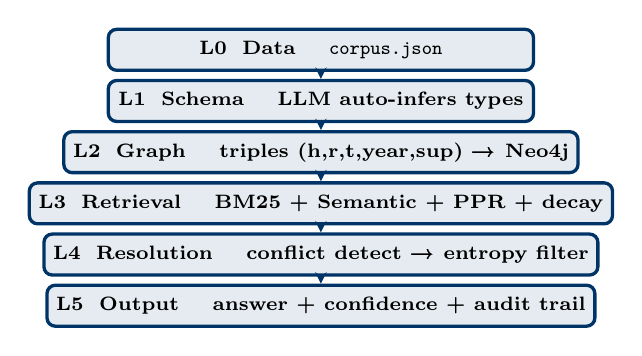
\begin{tikzpicture}[
    layer/.style={rectangle, draw=iiitblue, very thick,
                  fill=iiitblue!10, rounded corners=3pt,
                  minimum width=5.4cm, minimum height=0.52cm,
                  font=\scriptsize\bfseries, align=center},
    arr/.style={->, >=stealth, thick, color=iiitblue}
  ]
    \node[layer] (L0) at (0, 0)    {L0 \;Data \quad \texttt{corpus.json}};
    \node[layer] (L1) at (0,-0.65) {L1 \;Schema \quad LLM auto-infers types};
    \node[layer] (L2) at (0,-1.30) {L2 \;Graph \quad triples (h,r,t,year,sup) → Neo4j};
    \node[layer] (L3) at (0,-1.95) {L3 \;Retrieval \quad BM25 + Semantic + PPR + decay};
    \node[layer] (L4) at (0,-2.60) {L4 \;Resolution \quad conflict detect → entropy filter};
    \node[layer] (L5) at (0,-3.25) {L5 \;Output \quad answer + confidence + audit trail};
    \draw[arr](L0.south)--(L1.north); \draw[arr](L1.south)--(L2.north);
    \draw[arr](L2.south)--(L3.north); \draw[arr](L3.south)--(L4.north);
    \draw[arr](L4.south)--(L5.north);
  \end{tikzpicture}

  \vspace{6pt}
  \scriptsize
  \textbf{Score:}\;
  $s = R(p)\cdot\delta_h\cdot(1{+}\text{PPR})\cdot e^{-0.08t}\cdot(1{+}\ln(1{+}n){\cdot}0.8)$
\end{column}
% ── Right: tools + I/O ─────────────────────────────────────
\begin{column}{0.50\textwidth}
  \begin{block}{\small Tools Used}
    \scriptsize
    \begin{tabular}{ll}
      \toprule
      \textbf{Component} & \textbf{Tool} \\
      \midrule
      Language Model    & Qwen2.5-7B via Ollama (local) \\
      Graph Database    & Neo4j (Cypher queries) \\
      Embeddings        & Sentence-BERT all-MiniLM-L6-v2 \\
      Keyword Search    & BM25 (rank-bm25 library) \\
      LLM Framework     & LangChain \\
      Web API           & Flask REST \\
      Language          & Python 3.14 \\
      \bottomrule
    \end{tabular}
  \end{block}
  \vspace{4pt}
  \begin{block}{\small Input → Process → Output}
    \scriptsize
    \textbf{Input:} \texttt{corpus.json} (docs + queries)\\
    \textbf{Process:} Schema infer → graph build → hybrid\\
    \quad retrieve → conflict resolve → entropy filter\\
    \textbf{Output:} Answer + 0–100\% confidence + audit trail
  \end{block}
\end{column}
\end{columns}

\end{frame}

% ============================================================
% SLIDE 4 — Results & Analysis
% ============================================================
\begin{frame}{Slide 4 \quad Results \& Analysis}

\begin{columns}[T]
% ── Left: HaluEval ─────────────────────────────────────────
\begin{column}{0.47\textwidth}
  \begin{block}{\small HaluEval — 200 Questions (Hallucination)}
    \centering\scriptsize
    \begin{tabular}{lrrr}
      \toprule
      \textbf{System} & \textbf{HRR\%} & \textbf{EM\%} \\
      \midrule
      LangChain RAG          & 77.5 & 85.5 \\
      KG-RAG v4 (Simulated)  & 91.0 & 15.5 \\
      \rowV \textbf{v5 (Ours)}& \textbf{92.0} & 14.5 \\
      \bottomrule
    \end{tabular}
    \vspace{3pt}

    \raggedright
    \textbf{+14.5 pp} HRR over LangChain.\\
    LangChain's high EM = verbatim copying,\\
    not correct answers. HRR is the true metric.
  \end{block}
\end{column}
% ── Right: conflict benchmark ──────────────────────────────
\begin{column}{0.50\textwidth}
  \begin{block}{\small Conflict + Temporal — 125 Queries}
    \centering\scriptsize
    \begin{tabular}{lC{1.1cm}C{1.1cm}C{1.1cm}C{1.1cm}}
      \toprule
      \textbf{System} & \textbf{CDR\%} & \textbf{Temp\%} & \textbf{EM\%} & \textbf{Conf\%}\\
      \midrule
      LangChain  & 25.0 & 14.3 & 31.2 & --- \\
      KG-RAG v4  & 25.0 & 35.7 & 32.0 & --- \\
      \rowV \textbf{v5} & \textbf{50.0} & \textbf{35.7} & \textbf{33.6} & \textbf{29.4} \\
      \bottomrule
    \end{tabular}
    \vspace{3pt}

    \raggedright
    \textbf{CDR doubles} 25\%$\to$\textbf{50\%} — primary claim.\\
    \textbf{Temporal accuracy 2.5$\times$}: 14.3\%$\to$35.7\%.\\
    Only v5 produces a \textbf{calibrated confidence score}.
  \end{block}
\end{column}
\end{columns}

\vspace{6pt}
\centering\scriptsize
\begin{tabular}{lccc}
  \toprule
  & \textbf{LangChain} & \textbf{KG-RAG v4} & \textbf{TruthfulRAG v5}\\
  \midrule
  HRR\% (hallucination) & 77.5 & 91.0 & \textbf{92.0 (+14.5 pp)}\\
  CDR\% (conflict)      & 25.0 & 25.0 & \textbf{50.0 (2$\times$)}\\
  Temporal\%            & 14.3 & 35.7 & \textbf{35.7 (2.5$\times$)}\\
  \bottomrule
\end{tabular}

\end{frame}

% ============================================================
% SLIDE 5 — Conclusion
% ============================================================
\begin{frame}{Slide 5 \quad Conclusion}

\begin{columns}[T]
% ── Left: summary + key numbers ───────────────────────────
\begin{column}{0.46\textwidth}
  \begin{block}{\small Summary}
    \scriptsize
    \begin{itemize}\setlength\itemsep{3pt}
      \item Faithfully re-implemented KG-RAG v4 (arXiv:2511.10375)
      \item Added 6 novel contributions on top of v4
      \item Evaluated on 325 queries across 2 public benchmarks
      \item Runs \textbf{100\% offline} — no cloud, no cost,
            no data leakage
    \end{itemize}
  \end{block}
  \vspace{4pt}
  \begin{block}{\small Key Numbers}
    \scriptsize
    \begin{tabular}{ll}
      Score gap v4 $\to$ v5: & 0.028 $\to$ \textbf{1.126} \\
      HRR improvement:        & +14.5 pp over LangChain \\
      CDR improvement:        & 2$\times$ (25\% $\to$ 50\%) \\
      Temporal improvement:   & 2.5$\times$ (14.3\% $\to$ 35.7\%) \\
    \end{tabular}
  \end{block}
\end{column}
% ── Right: future scope + closing ─────────────────────────
\begin{column}{0.50\textwidth}
  \begin{block}{\small Future Scope}
    \scriptsize
    \begin{tabular}{L{2.5cm}L{3.2cm}}
      \toprule
      \textbf{Limitation} & \textbf{Fix Direction} \\
      \midrule
      Negation blindness  & Negation-aware fine-tuning \\
      Same-year conflicts & Source credibility score \\
      Fixed decay $\lambda$ & Domain-adaptive lambda \\
      Only 3 entropy samples & Semantic clustering \\
      \bottomrule
    \end{tabular}
  \end{block}
  \vspace{6pt}
  \centering
  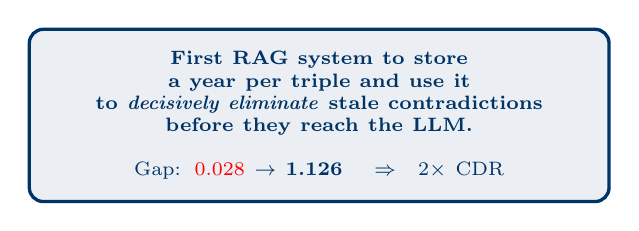
\begin{tikzpicture}
    \node[rectangle, draw=iiitblue, very thick, rounded corners=5pt,
          fill=iiitblue!8, text width=6.8cm, align=center, inner sep=8pt]{
      \scriptsize\bfseries\color{iiitblue}
      First RAG system to store a year per triple and use it\\
      to \emph{decisively eliminate} stale contradictions\\
      before they reach the LLM.\\[4pt]
      \normalfont Gap: \textcolor{red}{0.028} $\to$ \textbf{1.126}
      \quad$\Rightarrow$\quad 2$\times$ CDR
    };
  \end{tikzpicture}
\end{column}
\end{columns}

\end{frame}

% ============================================================
% SLIDE 6 — Key References
% ============================================================
\begin{frame}{Key References}

  \scriptsize
  \begin{thebibliography}{9}

    \bibitem{lewis2020rag}
    P.~Lewis \textit{et al.},
    ``Retrieval-Augmented Generation for Knowledge-Intensive NLP Tasks,''
    \textit{NeurIPS}, 2020.\\
    \textcolor{iiitblue}{\textbf{Role:}} Foundational RAG baseline —
    defines the architecture my system extends.

    \vspace{4pt}
    \bibitem{truthfulrag2024}
    Wang \textit{et al.},
    ``TruthfulRAG: Improving Factual Accuracy by Resolving Knowledge Conflicts,''
    \textit{arXiv:2511.10375}, 2024.\\
    \textcolor{iiitblue}{\textbf{Role:}} The paper I implemented as v4 and
    extended into v5 with 6 novel contributions.

    \vspace{4pt}
    \bibitem{ji2023survey}
    Z.~Ji \textit{et al.},
    ``Survey of Hallucination in Natural Language Generation,''
    \textit{ACM Computing Surveys}, 2023.\\
    \textcolor{iiitblue}{\textbf{Role:}} Peer-reviewed evidence that
    hallucination is a documented, real problem in LLMs.

    \vspace{4pt}
    \bibitem{halueval2023}
    J.~Li \textit{et al.},
    ``HaluEval: A Large-Scale Hallucination Evaluation Benchmark,''
    \textit{arXiv:2305.11747}, 2023.\\
    \textcolor{iiitblue}{\textbf{Role:}} Benchmark dataset used in
    Benchmark 1 (200 questions); v5 achieved 92\% HRR.

    \vspace{4pt}
    \bibitem{pan2024kg}
    S.~Pan \textit{et al.},
    ``Unifying LLMs and Knowledge Graphs: A Roadmap,''
    \textit{IEEE Trans.\ Knowledge and Data Eng.}, 2024.\\
    \textcolor{iiitblue}{\textbf{Role:}} Positions TruthfulRAG v5 within
    the broader LLM + Knowledge Graph research direction.

  \end{thebibliography}

\end{frame}

\end{document}
